\documentclass[tikz, border=3.14mm]{standalone}
\usepackage{pgfplots}
\pgfplotsset{compat=1.18}

\begin{document}
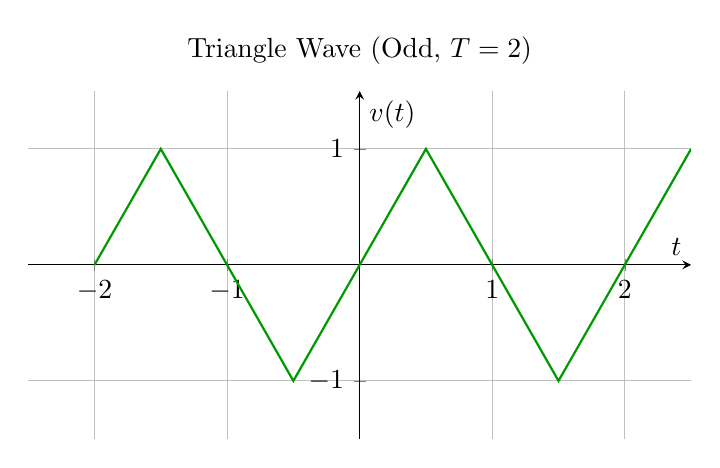
\begin{tikzpicture}
    \begin{axis}[
        axis lines = middle,
        xlabel = {$t$},
        ylabel = {$v(t)$},
        xmin = -2.5, xmax = 2.5,
        ymin = -1.5, ymax = 1.5,
        xtick = {-2, -1, 0, 1, 2},
        ytick = {-1, 1},
        grid = major,
        width = 10cm,
        height = 6cm,
        title = {Triangle Wave (Odd, $T=2$)}
    ]
        % Odd triangle wave: period 2, amplitude 1
        % Peak at t=0.5, Valley at t=1.5
        \addplot[green!60!black, thick, no marks] coordinates {
            (-2, 0)
            (-1.5, 1)
            (-0.5, -1)
            (0.5, 1)
            (1.5, -1)
            (2.5, 1)
        };
    \end{axis}
\end{tikzpicture}
\end{document}
